\documentclass{jsarticle}
\usepackage[dvipdfmx]{graphicx}
\usepackage{here}
\usepackage{listings}
\lstset{
    basicstyle={\ttfamily\small}, %書体の指定
    frame=tRBl, %フレームの指定
    framesep=10pt, %フレームと中身(コード)の間隔
    breaklines=true, %行が長くなった場合の改行
    linewidth=12cm, %フレームの横幅
    lineskip=-0.5ex, %行間の調整
    tabsize=2 %Tabを何文字幅にするかの指定
}
\begin{document}
\title{計算機科学実験2 ソフトウェア報告書1}
\author{新山公太(にいやまこうた)\\平成30年度入学\\1029300562}
\maketitle

\section{課題1}
\subsection{ステージパラメータの変更}
\subsubsection{seed値の変更}
seed値を変更すると、出てくる敵の種類に変化は見られずコースの地形のみに変化が見られた。また地形の変化というのもブロックのパターンに変化があるのみで、落とし穴が増えたり、土管の有無が変わったりすることはなかった。また敵の種類についてもseed値には影響されなかった。以下図1を見ることでステージ冒頭の地形が変わっていることが確認できる。

\begin{figure}[H]
	\begin{tabular}{c}
	\begin{minipage}{0.50\hsize}
		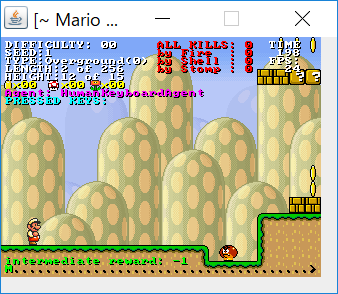
\includegraphics{seed1.png}
		\caption{seed値1のステージ冒頭}
	\end{minipage}
	\begin{minipage}{0.50\hsize}
		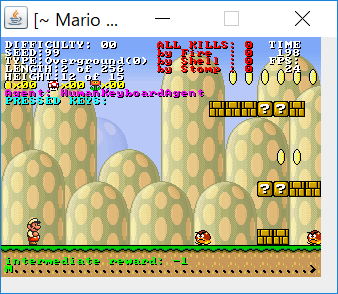
\includegraphics{seed99.png}
		\caption{seed値99のステージ冒頭}
	\end{minipage}
	\end{tabular}
\end{figure}

\subsubsection{難易度の設定}
資料に従ってステージの難易度を設定すると、地形に変化は見られず敵の数が多くなった。またデフォルトの設定では出てこなかった敵も出てきたので、一定の難易度以上でないと出現しない敵がいるのかもしれないと思って、後述する設定で出てくる敵を一種類に限定し難易度はデフォルトのままでプレイしてみたところ敵は出現したので、詳しいことはよくわからなかった。
また、キラー砲台などデフォルトのステージにはなかったものが増えることもあった。以下の図3と図2を見比べればキラー砲台が表れていることがわかる。

\begin{figure}
	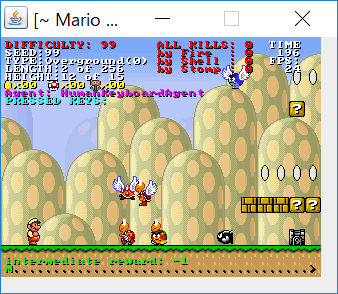
\includegraphics{difficulty99}
	\caption{難易度を99に設定したseed値99のステージ}
\end{figure}

\subsection{出てくる敵の指定}
資料に従い様々な敵について出現するかしないかを切り替えた。敵が出てこない設定にしても、パックンフラワーは出てきたがこれは土管がステージに現れないようにすれば解決できると思われる。また、現れる敵については数文字のアルファベットで指定するが、指定する順番を変えても出てくる敵の配置に変化は見られなかった。
\subsection{ForwardAgentの説明}
\subsubsection{reset()メソッドで行われていること}
このエージェントのreset()メソッドでは、コントローラのうち「右」と「ダッシュ」のボタンが押される。これはゲーム開始と同時にマリオに右に向かって走れという命令を出していることとなる。ここでは、それらのボタンを押すだけでなくtrueJumpCounterおよびtrueSpeedCounterという変数に0が代入されている。これら変数はgetAction()メソッドが呼び出されたときにそれぞれのボタンが押されている場合にインクリメントされていく。すなわちどれだけの間ボタンが押されていたかのパラメータとなっている。
\subsubsection{DangerOfAny()メソッドが返す真偽値}
このメソッドは名前の通り障害物がある場合や敵がいる場合にtrueを返すメソッドとなっている。具体的にはマリオの1マス前の地面が2マス以上何もない空間である、または、マリオの1マス前または2マス前が、何もない空間じゃない、または敵がいるときにtrueを返す。
すなわち目の前に段差や障害物があったり、敵がいたりするとtrueを返す。
\subsubsection{getAction()メソッドの説明}
このメソッドではDangerOfAny()メソッドがtrueを返していて、かつ目の前にある障害物がコインじゃないとき、ジャンプ可能であるかジャンプして空中にいるかならジャンプボタンを押し、目の前に障害物がないか障害物がコインの時、ジャンプボタンを離すという処理と、もしジャンプボタンを押したままgetAction()メソッドが15回呼び出されたらジャンプボタンを離すという処理の二つでボタンを押すか押さないかを決めている。要約すると、障害物と敵をジャンプで避け、できるだけ高く飛ぶようにしている。

\section{課題2}
\subsection{ステージをクリアするためのアイデア}
まずは資料にあった障害物をよけてゴールを目指すエージェントでMainTask2をプレイさせてみたところ、見事に落下した。(以下の図を参照)

\begin{figure}[H]
	\begin{tabular}{c}
	\begin{minipage}{0.50\hsize}
		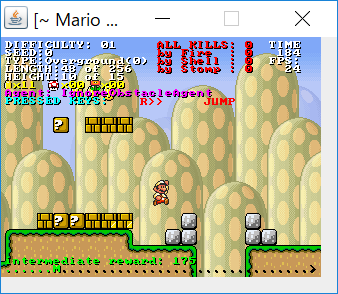
\includegraphics{falling1.png}
		\caption{落下するマリオ1}
	\end{minipage}
	\begin{minipage}{0.50\hsize}
		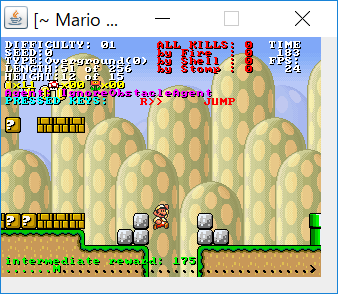
\includegraphics{falling2.png}
		\caption{落下するマリオ2}
	\end{minipage}
\\
	\begin{minipage}{0.06\hsize}
       	 \vspace{10mm}
      \end{minipage}
\\

	\begin{minipage}{0.50\hsize}
		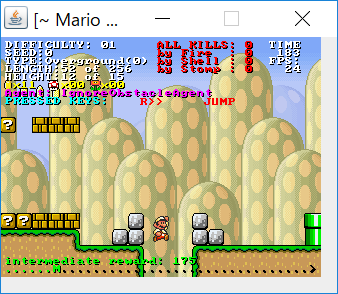
\includegraphics{falling3.png}
		\caption{落下するマリオ3}
	\end{minipage}
	\begin{minipage}{0.50\hsize}
		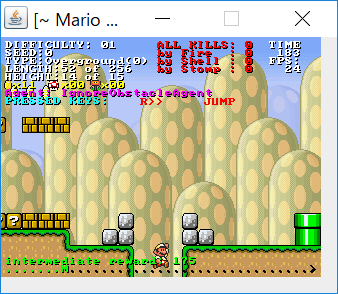
\includegraphics{falling4.png}
		\caption{落下するマリオ4}
	\end{minipage}
	\end{tabular}
\end{figure}
これは目の前の障害物を認識してジャンプボタンが押されたためである。このような事態を避けるためには穴に落ちそうなときそれ以上進まないようにすればよいと考えた。では、穴に落ちそうな時とはどのようなときだろうか。今回の図で考えてみればジャンプの飛距離が足りないことが落下の原因だと思われる。つまり、落とし穴をジャンプで避けようとするならば落とし穴の目の前でジャンプをするようにすればいいと考えた。そして飛距離が足りないときは、いったん落とし穴の目の前の足場に着地するようにすればよいのではないかと考えた。

\subsection{実装方法}
\subsection{落とし穴を発見する方法}
落とし穴があるかどうかを判定するために、ステージの空間を縦に見ていき、マリオより低い位置に足場がないときにtrueを返すメソッドを作った。このメソッドにはint型の整数を渡すことで、マリオから見てその分だけ先の位置に落とし穴があるかどうかを判定することができる。
\subsection{危ないときに進まないようにする方法}
最初は目の前が落とし穴、かつマリオから見て(0,1)進んだ座標が足場になっているときに左に進むボタンを押すことで進まないようにしていた。しかしこの実装方法ではMainTask2でseed値17の時に落とし穴に落ちてしまう。(以下の図を参照)

\begin{figure}[H]
	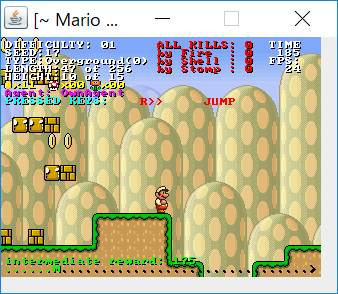
\includegraphics{falling_hole}
	\caption{最初の実装で越えられない落とし穴}
\end{figure}

このような状況を避けるために、実装方法を少し変えた。このプログラムではマリオから見た座標ではない絶対座標といえる情報を取得することができる。今回はその情報を使うことでマリオが落下中かどうかを判定するメソッドを作った。これはgetAction()メソッドが毎フレームごとに呼び出されるのを利用することで可能であった。マリオが落下中で目の前に落とし穴があるときマリオは一度その場に着地するように左のボタンが押される。そうすることで、マリオは一度地面に着地してから万全の状態で落とし穴を飛び越えることができる。実際にはさらに万全を期すために落とし穴の上を通っているときにはダッシュボタンも押すようにしている。
\newpage
\subsection{stdout}
\begin{lstlisting}
[~ Mario AI Benchmark ~ 0.1.9]

[MarioAI] ~ Evaluation Results for Task: BasicTask
        Evaluation lasted : 47972 ms
         Weighted Fitness : 7200
             Mario Status : WIN!
               Mario Mode : FIRE
Collisions with creatures : 0
     Passed (Cells, Phys) : 256 of 256, 4096 of 4096 (100% passed)
 Time Spent(marioseconds) : 78
  Time Left(marioseconds) : 122
             Coins Gained : 65 of 227 (28% collected)
      Hidden Blocks Found : 0 of 0 (0% found)
       Mushrooms Devoured : 0 of 0 found (0% collected)
         Flowers Devoured : 0 of 2 found (0% collected)
              kills Total : 0 of 0 found (0%)
            kills By Fire : 0
           kills By Shell : 0
           kills By Stomp : 0
    PunJ : 0

 min = 0.0
 max = 0.0
 ave = 0.0
 sd  = NaN
 n   = 1
\end{lstlisting}

\end{document}